\section{Linear Regression} %4.2

In the first algorithm, Linear Regression model provides a basic fitting results. Without the addition of penalty term, $\text{R}^2$ reached 0.8982 (as Figure \ref{4.2.1-LR-Training-Results} shown), the mean square error (MSE) reached 0.00946 when the test set was used for evaluation.

\begin{table}[htbp]
  \centering
  \footnotesize
  \begin{tabular}{p{5.75cm} | c c c c c c}
  \toprule
  Coefficients: \\ %row 1
    & Estimate & Std. Error & t value & $\text{Pr}(>|\text{t}|)$\\
  \hline
  (Intercept) & 0.72626 & 0.02602 & 27.912 & $< \text{2e-16}$ & ***\\
  Rainfall & 0.04478 & 0.02495 & 1.799 & 0.0727 & .\\
  Daylight & 0.18852 & 0.03376 & 5.583 & $\text{3.95e-08}$ & ***\\
  Population & -0.98423 & 0.13192 & -7.461 & $\text{4.07e-13}$ & ***\\
  CO2 & 1.86621 & 0.19379 & 9.630 & $< \text{2e-16}$ & ***\\
  Ozone & 0.39157 & 0.03262 & 12.003 & $< \text{2e-16}$ & ***\\
  OceanTemperature\_NorthernHemisphere & -0.23312 & 0.04408 & -5.289 & $< \text{1.87e-07}$ & ***\\
  LandTemperature\_NorthernHemisphere & 0.08561 & 0.03910 & 2.190 & 0.0290 & *\\
  MinTemperature\_NorthSlopeAlaska & -0.63691 & 0.05038 & -12.642 & $< \text{2e-16}$ & ***\\
  GDP\_WORLD & -69403 & 0.07102 & -9.772 & $< \text{2e-16}$ & ***\\
  \hline
  \multicolumn{6}{l}{Signif. codes: 0 '***' 0.001 '**' 0.01 '*' 0.05 '.' 0.1 '' 1} \\
  \multicolumn{6}{l}{Residual standard error: 0.08382 on 480 degrees of freedom}\\
  \multicolumn{6}{l}{   15894 observations deleted due to missingness}\\
  \multicolumn{6}{l}{Multiple R-squared: 0.8982,      Adjusted R-squared: 0.8963}\\
  \multicolumn{6}{l}{F-statistic: 470.5 on 9 and 480 DF, P-value: $< \text{2e-16}$}\\
  \bottomrule
  \end{tabular}
  \caption{Linear Regression training results.}
  \label{4.2.1-LR-Training-Results}
\end{table}


\begin{figure}[htbp]
\centering
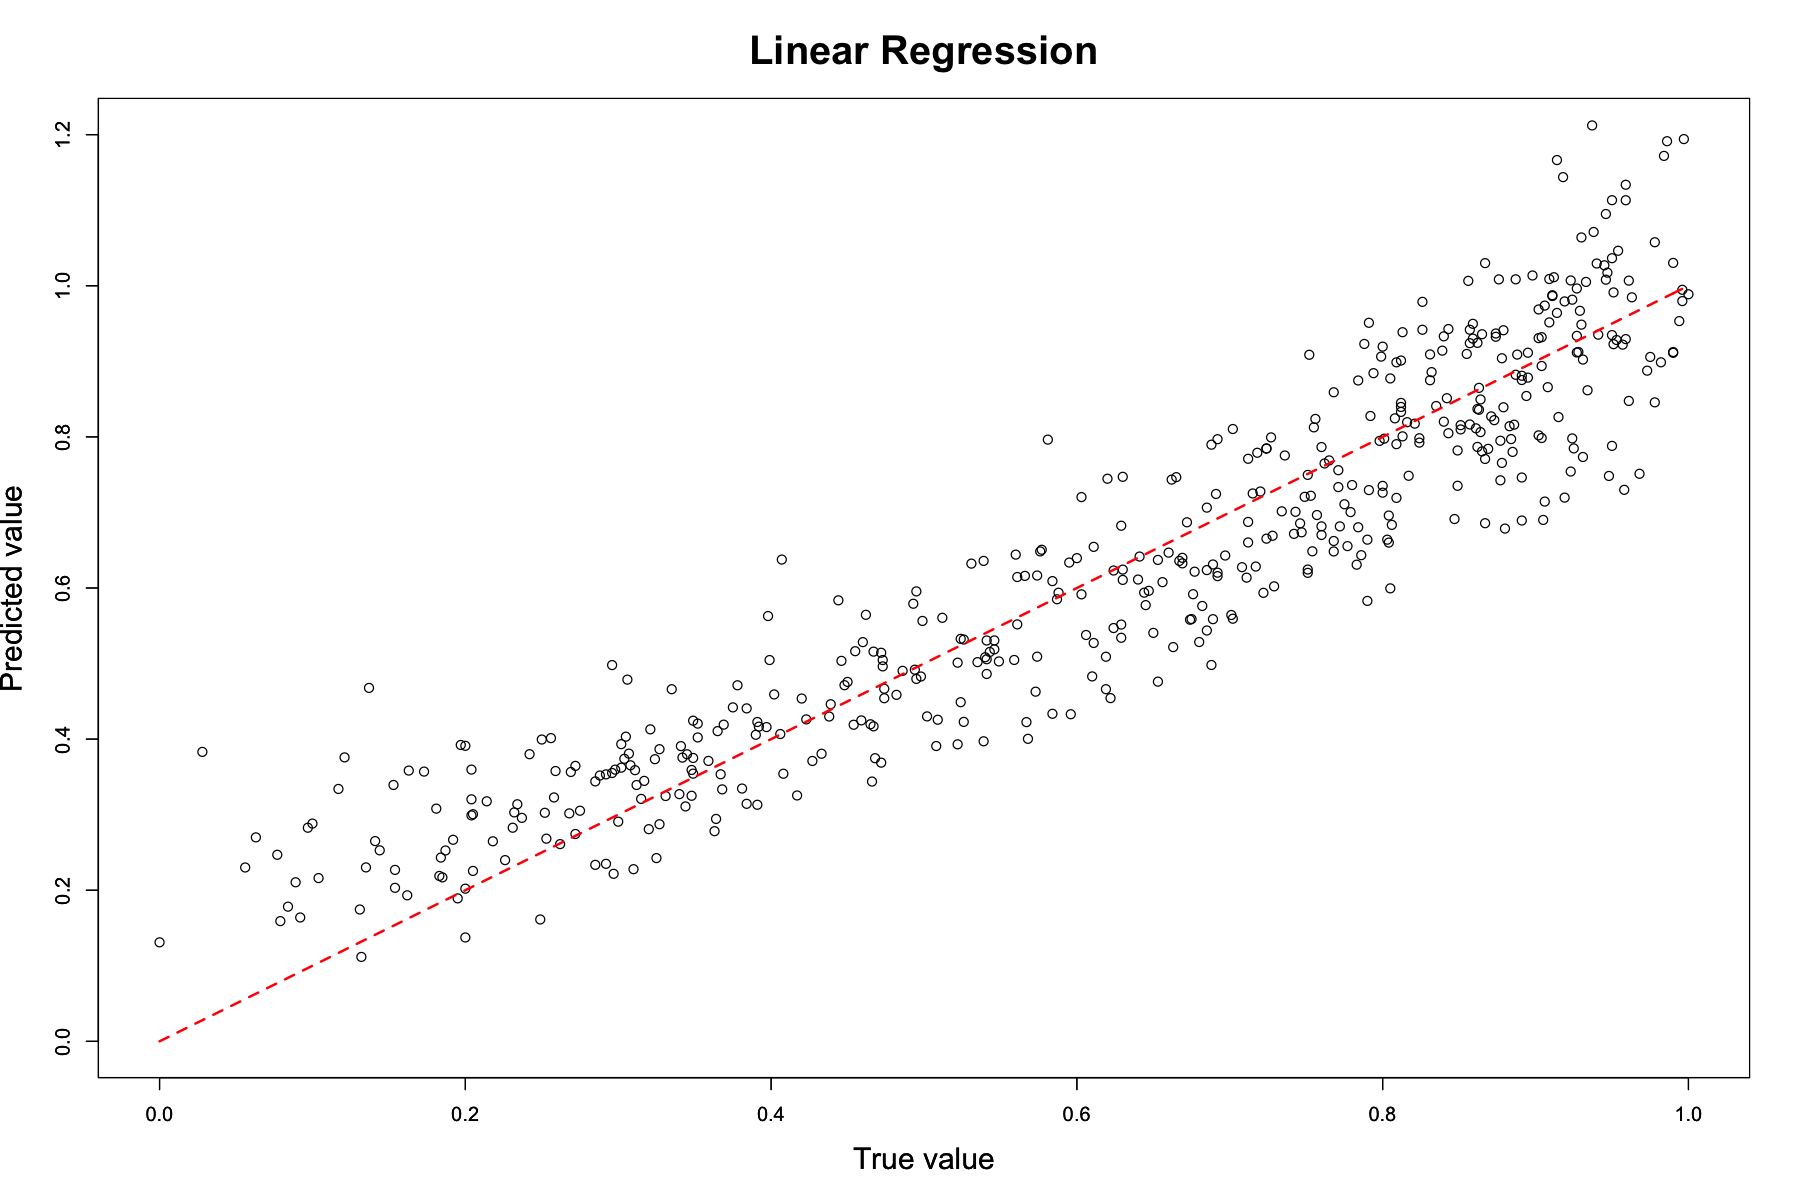
\includegraphics[width = 1.0\textwidth]{Figure/4.2.1-LR.png}
\caption{The predicted Arctic sea ice extent value vs the real Arctic sea ice extent value with \textbf{Linear Regression}. The red referenced dotted line represents the straight line y=x. Mean Square Error (MSE) is \textbf{0.00946}.}
\label{4.2.1-LR}
\end{figure}

Fitting diagram was generated as Figure \ref{4.2.1-LR}. It shows that the fitting points are not concentrated around the straight line $y=x$. In fact, this prediction was over-fitting. Comparing to other models that will be discussed later, the MSE of Linear Regression is relatively bigger, which means Linear Regression cannot predict the sea ice very well.

\newpage